\chapter{KIẾN TRÚC HỆ THỐNG TỔNG THỂ}

\section{Sơ đồ kiến trúc tổng quát}
Hệ thống TourXport được thiết kế dựa trên kiến trúc client-server hiện đại, phân tách rõ ràng giữa các lớp xử lý nhằm đảm bảo tính mở rộng và dễ dàng bảo trì. Kiến trúc tổng quát bao gồm ba thành phần chính:

\begin{itemize}
    \item \textbf{Lớp ứng dụng (Client-side):} Được xây dựng bằng framework Flutter, đóng vai trò là giao diện tương tác trực tiếp với người dùng. Thành phần này chịu trách nhiệm thu thập yêu cầu, hiển thị dữ liệu và quản lý trạng thái ứng dụng.
    \item \textbf{Lớp dịch vụ (Server-side):} Sử dụng môi trường Node.js \cite{nodejs} và framework Express \cite{expressjs}. Lớp này đóng vai trò trung tâm điều phối, xử lý các logic nghiệp vụ, xác thực người dùng và giao tiếp với các dịch vụ bổ trợ.
    \item \textbf{Lớp dịch vụ AI (AI Backend):} Một hệ thống riêng biệt chuyên trách xử lý các yêu cầu liên quan đến mô hình ngôn ngữ lớn (LLM) và kỹ thuật RAG (Retrieval-Augmented Generation) để cung cấp các gợi ý hành trình cá nhân hóa.
    \item \textbf{Lớp lưu trữ (Database):} Sử dụng MongoDB \cite{mongodb} để lưu trữ dữ liệu dưới dạng tài liệu (Document-oriented), cho phép cấu trúc dữ liệu linh hoạt phù hợp với các thông tin du lịch đa dạng.
\end{itemize}

\begin{figure}[H]
    \centering
    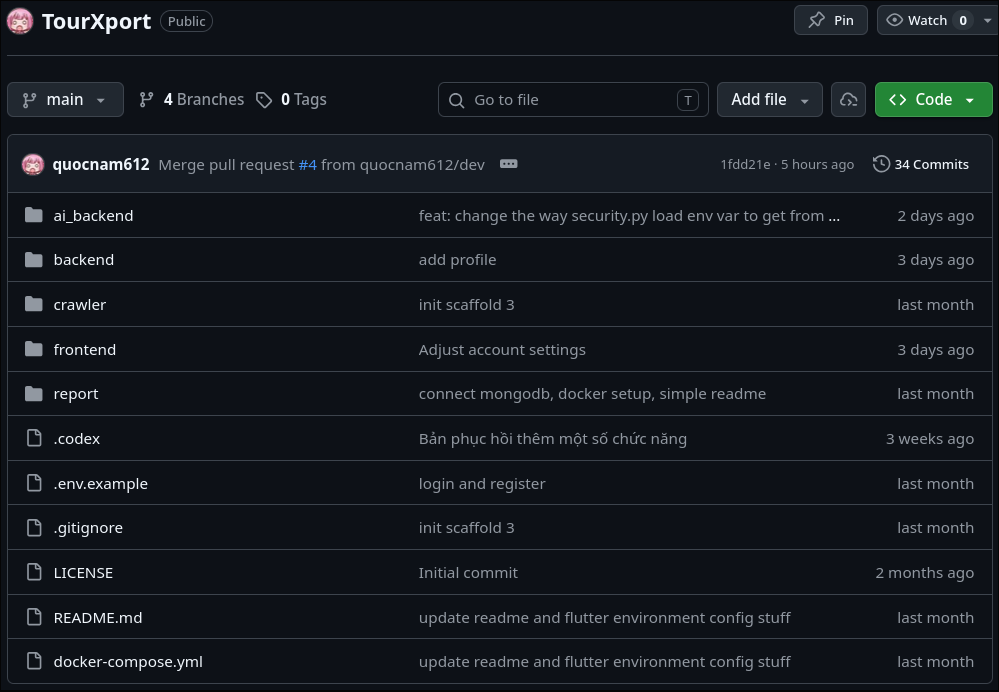
\includegraphics[width=0.6\textwidth]{img/C2-3.png}
    \caption{Kiến trúc thư mục của dự án TourXport}
\end{figure}

\section{Luồng giao tiếp giữa các thành phần}
Luồng dữ liệu trong hệ thống được thực hiện thông qua giao thức HTTP/HTTPS với định dạng dữ liệu chuẩn JSON. Quy trình tương tác điển hình được thực hiện qua các bước sau:

\begin{enumerate}
    \item \textbf{Gửi yêu cầu:} Client gửi yêu cầu kèm theo mã xác thực JWT (JSON Web Token) đến các điểm cuối (endpoints) tương ứng trên Backend Server.
    \item \textbf{Xử lý tại Backend:} Server thực hiện kiểm tra quyền truy cập thông qua các Middleware. Tùy theo loại yêu cầu, server sẽ truy vấn trực tiếp vào cơ sở dữ liệu hoặc gửi tiếp yêu cầu đến dịch vụ AI.
    \item \textbf{Xử lý AI và Dữ liệu:} Dịch vụ AI tiếp nhận yêu cầu, thực hiện truy xuất dữ liệu từ các nguồn đã được chuẩn hóa (Scraped data) để tạo ra phản hồi thông minh.
    \item \textbf{Phản hồi:} Kết quả được đóng gói và trả về Client. Lớp ứng dụng thực hiện giải mã JSON và cập nhật giao diện người dùng ngay lập tức.
\end{enumerate}

\begin{figure}[H]
    \centering
    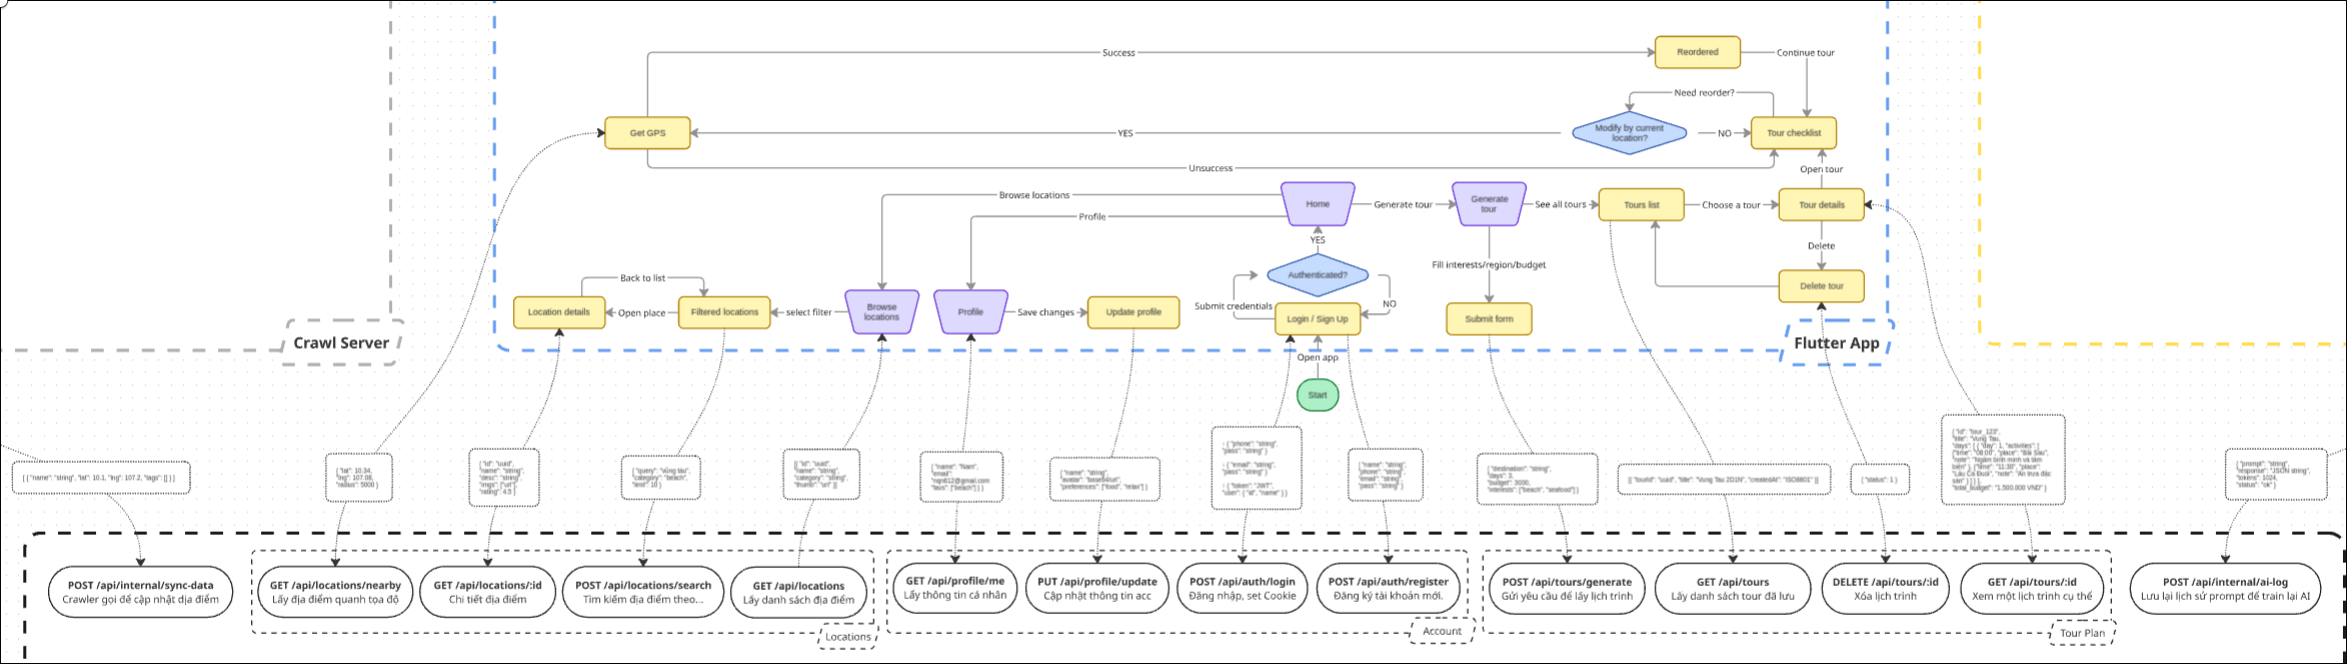
\includegraphics[width=1\textwidth]{img/C2-1.png}
    \caption{Sơ đồ luồng giao tiếp giữa các thành phần của hệ thống TourXport}
\end{figure}

\section{Thiết kế Cơ sở dữ liệu tập trung trên MongoDB}
Cơ sở dữ liệu được thiết kế theo mô hình tập trung, tận dụng khả năng lưu trữ không cấu trúc của MongoDB để tối ưu hóa tốc độ truy xuất. Các thực thể chính bao gồm:

\subsection{Cấu trúc người dùng (User Collection)}
Lưu trữ thông tin định danh, thông tin cá nhân và các cài đặt bảo mật. Mật khẩu được mã hóa trước khi lưu trữ để đảm bảo an toàn dữ liệu.

\subsection{Cấu trúc hành trình (Tour Collection)}
Đây là thành phần cốt lõi của hệ thống, lưu trữ các Tour được tạo ra bởi AI. Cấu trúc bao gồm các mảng lồng nhau (Nested Arrays) để biểu diễn lịch trình theo từng ngày, bao gồm địa điểm, thời gian dự kiến và chi phí ước tính.

\subsection{Cấu trúc địa điểm (Place Collection)}
Chứa dữ liệu đã qua xử lý được thu thập bởi Data Engineer, bao gồm tọa độ địa lý, mô tả chi tiết, hình ảnh và đánh giá chất lượng. Việc tập trung hóa dữ liệu địa điểm giúp giảm độ trễ khi AI thực hiện truy xuất thông tin (RAG).

\begin{figure}[H]
    \centering
    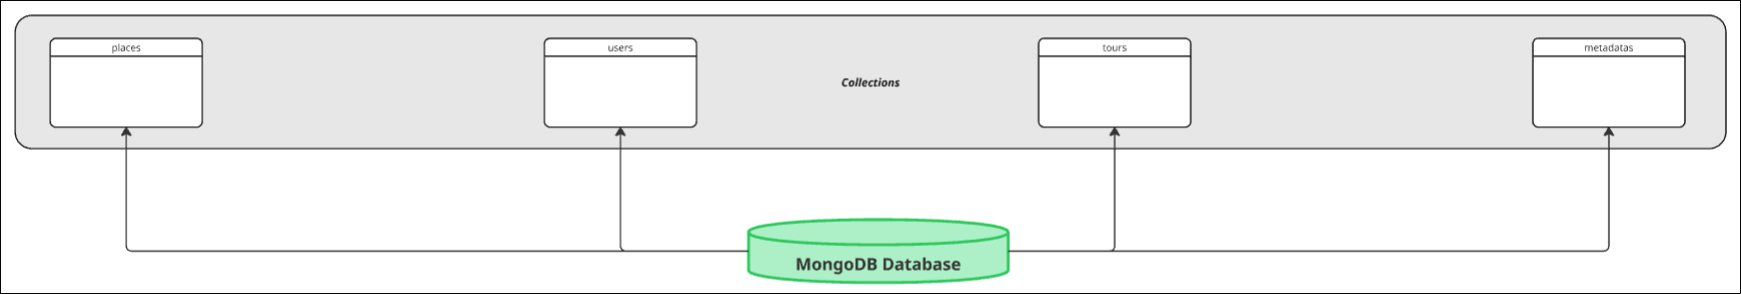
\includegraphics[width=1\textwidth]{img/C2-2.png}
    \caption{Sơ đồ thiết kế cơ sở dữ liệu trên MongoDB}
\end{figure}